\documentclass[11pt, letterpaper]{article}

% Essential Packages
\usepackage[utf8]{inputenc}
\usepackage{geometry}
\geometry{margin=1in}
\usepackage{amsmath, amssymb, amsfonts} % Math packages
\usepackage{graphicx} % For images
\usepackage{hyperref} % For clickable links
\usepackage{physics} % Partial derivatives and notation
\usepackage{fancyhdr} % Headers and footers
\usepackage{parskip}  % Adds space between paragraphs instead of indentation
\usepackage{float}
\usepackage[export]{adjustbox}

% Title Information
\title{\textbf{Physics of a Circular Membrane}\\ \large Derivation and Analysis of the 2D Wave Equation}
\author{Eben Quenneville \\ Classical Mechanics II / PHYS 616}
\date{\today}

\begin{document}

\maketitle

\begin{abstract}
    In this project, we examine the physics of a drum head modeled as a circular membrane under uniform tension. We derive the two-dimensional wave equation from Newton's Second Law and transform the problem into polar coordinates. Using the method of separation of variables, we solve the equations of motion in terms of Bessel functions. Finally, we examine the time evolution of the membrane under various initial conditions and provide visualizations.
\end{abstract}

\tableofcontents
\newpage

\section{Introduction}

The vibration of a drum head is a classic problem in mathematical physics. By modeling the drum as a membrane with tension applied at a circular boundary, we derive the standard 2D wave equation. The solutions to this PDE provide deep insight into acoustic physics, introducing the concept of normal modes and Bessel functions. This report details the analytic derivation and provides a framework for programmatic visualization of arbitrary initial conditions.

\section{Governing Equations}

Consider a elastic circular membrane of radius $a$, perturbed from its rest state and allowed to oscillate.
We seek an equation to govern the evolution of the membrane over time.
To allow for analytic solutions, we make several physical assumptions:
\begin{enumerate}
    \item The membrane is a perfectly elastic, infinitesimally thin sheet with surface mass density $\sigma$.
    \item It is clamped rigidly along the boundary, resulting in constant, uniform tension per unit length, $T$.
    \item Damping effects due to air resistance and internal friction are neglected.
\end{enumerate}

The governing equation arises from Newton's Second Law. Consider a differential square patch of the membrane. Let $z = u(x, y, t)$ describe the vertical displacement of the membrane from the rest plane $z = 0$.

When displaced, the surface curvature causes the tension forces on opposing sides of the patch to misalign, creating a net vertical restoring force. Let the patch range from $x$ to $x + \Delta x$ and $y$ to $y + \Delta y$, with mass $m = \sigma \Delta x \Delta y$. Denote the angles of inclination between the tension and the horizontal be $\alpha$ and $\beta$ in a cross-sectional view, as depicted in Figure \ref{fig:membrane_force}.

\begin{figure}[h]
    \centering
    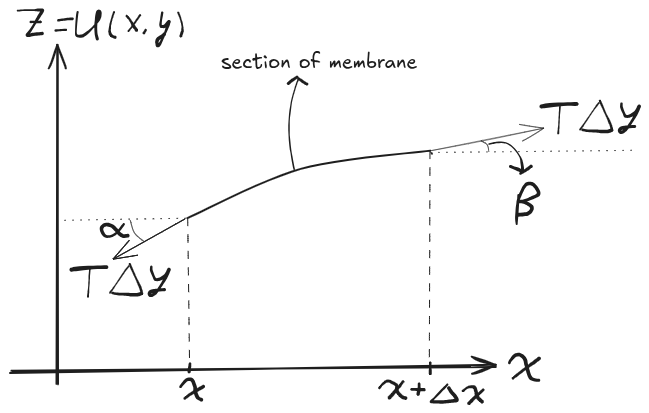
\includegraphics[width=0.6\textwidth]{src/membrane_example.excalidraw.png} 
    \caption{A differential patch of the membrane in the $xz$-plane. The tension $T$ acts at angles $\alpha$ and $\beta$, creating a net vertical restoring force.}
    \label{fig:membrane_force}
\end{figure}

For small displacements, we assume the angles of inclination $\alpha$ and $\beta$ are small, such that $\sin(\alpha) \approx \tan(\alpha) \approx \pdv{u}{x}$. The vertical component of tension is approximately $T \pdv{u}{x}$. An analogous argument can be made in the $yz$ plane, where instead $\sin(\alpha) \approx \pdv{u}{y}$. Then, summing the forces on all sides:

\begin{equation}
F_z = T\left[\Delta y \frac{\partial u}{\partial x}(x + \Delta x, y) - \Delta y \frac{\partial u}{\partial x}(x, y) + \Delta x \frac{\partial u}{\partial y}(x, y + \Delta y) - \Delta x \frac{\partial u}{\partial y}(x, y)\right]
\end{equation}

Applying the multivariable Taylor series approximation, where $\pdv{u}{x}(x + \Delta x, y) \approx \pdv{u}{x}(x, y) + \pdv[2]{u}{x}(x, y) \Delta x$, the force equation simplifies to:
\begin{align}
F_z &= \Delta x \Delta y T \left(\pdv[2]{u}{x} + \pdv[2]{u}{y}\right)
\end{align}
Applying Newton's Second Law ($F = ma$):
\begin{align}
    (\sigma \Delta x \Delta y) \pdv[2]{u}{t} &= \Delta x \Delta y T \left( \pdv[2]{u}{x} + \pdv[2]{u}{y} \right) \\
    \pdv[2]{u}{t} &= \frac{T}{\sigma} \nabla^2 u
\end{align}

It is convention to define $c = \sqrt{\frac{T}{\sigma}}$, which is the speed at which a wave is capable of propagating through our elastic membrane. 

We thus arrive at the classical wave equation:
\begin{equation}
    \boxed{\pdv[2]{u}{t} = c^2 \nabla^2 u}
    \label{eq:wave_eqn_cartesian}
\end{equation}

\section{Transformation to Polar Coordinates}

Equation \ref{eq:wave_eqn_cartesian} is the general wave equation. However, our boundary conditions for a drum are circular ($x^2 + y^2 = a^2$). It is thus advantageous to switch to polar coordinates $(r, \theta)$, where the circle can be described by the equation $r = a$. The Laplacian in polar coordinates (see Appendix A) is:
\begin{equation}
    \nabla^2 = \frac{1}{r} \pdv{r} \left( r \pdv{r} \right) + \frac{1}{r^2} \pdv[2]{\theta}
\end{equation}
Thus, the governing PDE becomes:
\begin{equation}
    \boxed{\frac{1}{r} \pdv{r} \left( r \pdv{u}{r} \right) + \frac{1}{r^2} \pdv[2]{u}{\theta} = \frac{1}{c^2} \pdv[2]{u}{t}}
    \label{eq:wave_eqn_polar}
\end{equation}

\pagebreak

\section{Constraints and Conditions}

To solve Equation \ref{eq:wave_eqn_polar}, we impose the following conditions:
\begin{itemize}
    \item \textbf{Dirichlet Boundary Condition:} The drum is fixed at the rim.
    \begin{equation}
        u(a, \theta, t) = 0 \quad \forall\, \theta, t
    \end{equation}
    \item \textbf{Periodicity:} The solution must be continuous around the circle.
    \begin{equation}
        u(r, \theta, t) = u(r, \theta + 2\pi, t)
    \end{equation}
    \item \textbf{Initial Conditions:}
    \begin{equation}
        u(r, \theta, 0) = f(r, \theta), \quad \pdv{u}{t}(r, \theta, 0) = g(r, \theta)
    \end{equation}
\end{itemize}

In this framework our goal is thus to find $u$ given initial deformation of the membrane $f$ and velocity $g$.

\section{Fundamental Modes via Separation of Variables}

To solve, we assume a separable solution of the form:
\begin{equation}
    u(r, \theta, t) = R(r) \Theta(\theta) T(t)
\end{equation}

By assuming this form, we imply that the spatial profile of the oscillation is decoupled from its temporal evolution. 
This describes a \textit{standing wave}, where the nodal lines (points of zero displacement) remain fixed in space while the amplitude oscillates. 
We shall later write the general solution as a superposition of these fundamental standing wave modes.

Substituting this into the wave equation and dividing by $R\Theta T$:
\begin{equation}
    \frac{1}{R r} \pdv{r} \left(r \dv{R}{r}\right) + \frac{1}{r^{2} \Theta} \dv[2]{\Theta}{\theta} = \frac{1}{c^{2}T} \dv[2]{T}{t}
\end{equation}
Since the left side depends only on space and the right only on time, both must equal a constant, which we denote $-\lambda^2$.

\subsection{Time Dependence}

The time component satisfies a harmonic oscillator equation:
\begin{equation}
    \dv[2]{T}{t} + c^2\lambda^2 T = 0 \implies \dv[2]{T}{t} + \omega^2 T = 0
\end{equation}
where $\omega = c\lambda$. The solution is:
\begin{equation}
    T(t) = A \cos(\omega t) + B \sin(\omega t)
\end{equation}

\subsection{Spatial Dependence}

Separating the radial and angular components:

\begin{equation}
    \frac{r}{R} \pdv{r} \left(r \dv{R}{r} \right) + \lambda^{2} r^{2} = - \frac{1}{\Theta} \dv[2]{\Theta}{\theta} = m^2
\end{equation}

The angular equation $\Theta'' + m^2\Theta = 0$ yields periodic solutions only if $m$ is an integer. Thus:

\begin{equation}
    \Theta_m(\theta) = C_m \cos(m\theta) + D_m \sin(m\theta), \quad m = 0, 1, 2, \dots
\end{equation}

The radial equation becomes \textbf{Bessel's Differential Equation}:

\begin{equation}
    r^2 R'' + r R' + (\lambda^2 r^2 - m^2)R = 0
\end{equation}

The general solution involves Bessel functions of the first ($J_m$) and second ($Y_m$) kind:
\begin{equation}
    R(r) = c_1 J_m(\lambda r) + c_2 Y_m(\lambda r)
\end{equation}

Since $Y_m(\lambda r) \to -\infty$ as $r \to 0$, we must set $c_2 = 0$ to maintain physical viability at the center of the drum. See Appendix B for details on the Bessel functions.

\subsection{Eigenfrequencies}
Applying the boundary condition $R(a) = J_m(\lambda a) = 0$, we see that $\lambda a$ must be a root of the Bessel function. Letting $\alpha_{mn}$ be the $n$-th zero of $J_m$, the allowable wavenumbers are $\lambda_{mn} = \alpha_{mn}/a$.

The general solution is a superposition of these modes:
\begin{equation}
	\boxed{\begin{aligned}
u(r, \theta, t) = \sum_{m=0}^{\infty} \sum_{n=1}^{\infty} J_{m}(\lambda_{mn} r) \Big[ &(A_{mn} \cos m \theta + B_{mn} \sin m \theta )\cos \omega_{mn} t \\
&+ (C_{mn} \cos m \theta + D_{mn} \sin m \theta) \sin \omega_{mn} t \Big]
\end{aligned}}
\end{equation}

\section{Coefficient Determination}

The coefficients are determined using the orthogonality of Bessel functions and trigonometric functions.

Let $u(r, \theta, 0) = f(r, \theta)$ be the initial position of the drum. The terms involving $\sin(\omega_{mn}t)$ vanish at $t = 0$, and the cosine terms become 1. Thus,

\begin{equation}
f(r, \theta) = \sum\limits_{m=0}^{\infty}\sum\limits_{n=1}^{\infty} J_{m}(\lambda_{mn} r) [A_{mn} \cos(m \theta) + B_{mn} \sin(m \theta)]
\end{equation}
We know from earlier in the semester that the inner product of $\cos(m \theta)$ and $\cos(n \theta)$ is 0 if $m \neq n$, and similarly for sines. So, we can separate the $m$th term by multiplying our equation by $\cos(m \theta)$ or $\sin(m \theta)$ and integrating from $0$ to $2 \pi$. In particular,
\begin{equation}
\int\limits_{0}^{2\pi}{f(r, \theta) \cos(m \theta)d \theta} = \pi \sum\limits_{n=1} A_{mn} J_{m}(\lambda_{mn} r)
\end{equation}
Note that if $m = 0$, the factor is $2 \pi$ instead of $\pi$. 

We are now left with a series of Bessel functions. By construction, the Bessel functions $J_{m}(\lambda_{mn} r)$ form an orthogonal set on $[0, a]$, with respect to the weight function $w(r) = r$. So 

\begin{equation}
\int\limits_{0}^{a}{J_{m}(\lambda_{mn} r) J_{m}(\lambda_{mp}) r dr} = \begin{cases}
0 & \text{if } n \neq p\\
\frac{a^{2}}{2} [J_{m+1}(\alpha_{mn})]^{2} &\text{if } n = p
\end{cases}
\end{equation}

where still $\alpha_{mn} = \lambda_{mn} a$ is a zero of the $m$-th Bessel function. So, we take the result from angular integration, and multiply by $J_{m}(\lambda_{mn} r) \cdot r$ and integrate from $0$ to $a$:

\begin{equation}
\int\limits_{0}^{a} \left[ \int\limits_{0}^{2\pi}{f(r, \theta) \cos(m \theta)d \theta}\right] J_{m} (\lambda_{mn}r)r ~dr = \pi A_{mn} \frac{a^{2}}{2} J_{m+1}^{2} (\alpha_{mn})
\end{equation}

We then rearrange for $A_{mn}$ to get

\begin{equation}
A_{mn} = \frac{2}{\pi a^{2} J_{m+1}^{2} (\alpha_{mn})} \int\limits_{0}^{a} \int\limits_{0}^{2 \pi}{f(r, \theta) J_{m}(\lambda_{mn} r) \cos(m \theta) r ~dr ~d \theta}
\end{equation}

The exact same logic for the sine terms resolves $B_{mn}$ to be 

\begin{equation}
B_{mn} = \frac{2}{\pi a^{2} J_{m+1}^{2}(\alpha_{mn})} \int\limits_{0 }^{a} \int\limits_{0}^{2 \pi}{f(r, \theta) J_{m}(\lambda_{mn} r) \sin(m \theta)r ~dr ~d \theta}
\end{equation}

Finally, to find $C_{mn}$ and $D_{mn}$, we use the initial velocity condition $\frac{\partial u}{\partial t} = g(r, \theta)$ for some function $g$. Taking the time derivative will bring down an extra constant factor of $\omega_{mn}$. So, we get 

\begin{equation}
C_{mn} = \frac{2}{\pi a^{2} \omega_{mn} J_{m+1} ^{2}(\alpha_{mn})} \int\limits_{0}^{a} \int\limits_{0}^{2\pi} g(r, \theta) J_{m}(\lambda_{mn}r) \cos(m \theta) r ~dr ~d \theta
\end{equation}

and 

\begin{equation}
D_{mn} = \frac{2}{\pi a^{2} \omega_{mn} J_{m+1}^{2}(\alpha_{mn})} \int\limits_{0}^{a} \int\limits_{0}^{2 \pi}{g(r, \theta) J_{m}(\lambda_{mn} r) \sin(m \theta) r ~ dr ~d \theta}
\end{equation}

With this, we have the full mathematical framework complete.

\section{Programmatic Approach and Visualization}

With the mathematical framework in place, the solutions can be visualized using the Julia programming language.
All code can be found in the \href{https://github.com/TonehavenE/PHYS616_Final_project}{project GitHub}.

\subsection{Normal Modes}

Earlier, it was claimed that any arbitrary configuration of the drum could be represented by a sum of normal modes.
We now visualize the fundamental modes, defined by $\psi_{mn} = J_m(\lambda_{mn}r)\cos(m\theta)$. 
We neglect time dependence and include only one trigonometric multiplier since $\sin$ would just rotate the mode.
Figure \ref{fig:modes} displays the first several modes.
Note that $m$ determines the number of nodal diameters, and $n$ determines the number of nodal circles.

\begin{figure}[H]
    \centering
    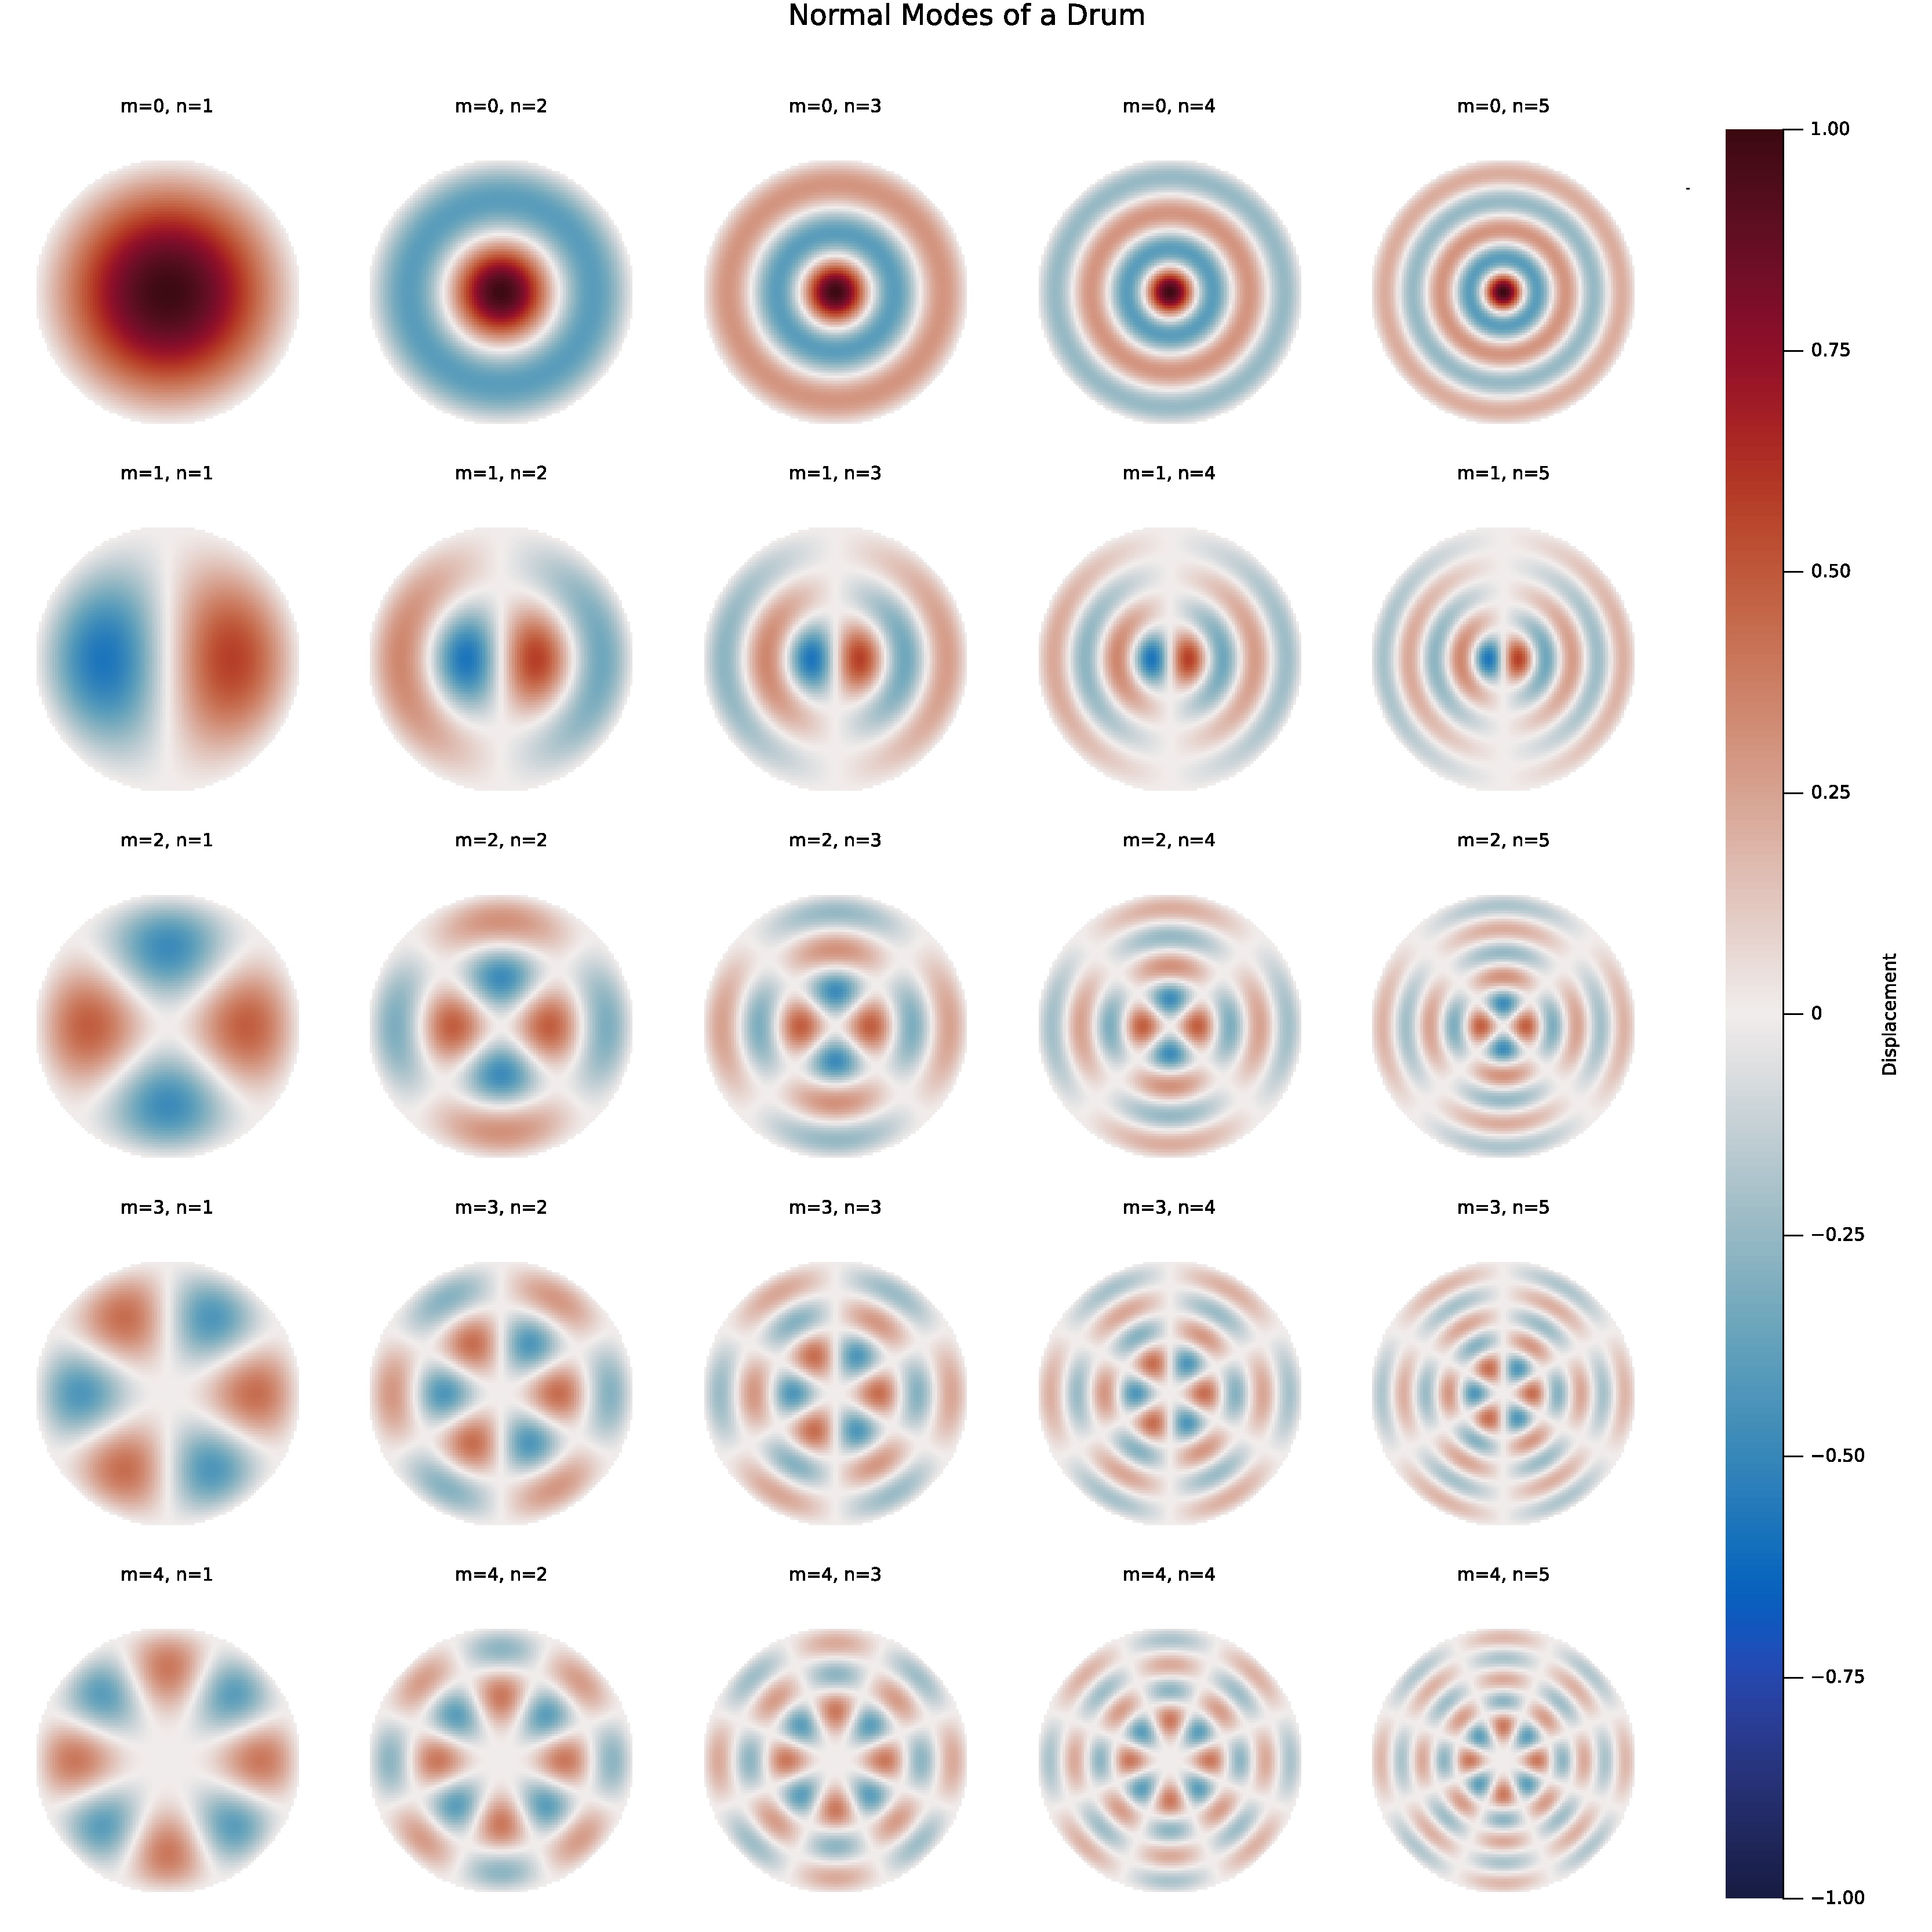
\includegraphics[width=0.8\textwidth]{src/normal_modes.pdf}
    \caption{Grid of the first several normal modes of the circular membrane.}
    \label{fig:modes}
\end{figure}

This can also be visualized as an animation, which is seen in the notebook.

\subsection{Time Evolution}
Next, we can visualize how a particular initial condition of a drum would evolve with time.
We simulate the evolution of a Gaussian pulse initially centered at the origin in Figure \ref{fig:gaussian}:
\begin{equation}
    f_{\text{init}}(r, \theta) = \frac{1}{2} e^{-20r^2}, \quad g_{\text{init}} = 0
\end{equation}
\begin{figure}[H]
    \centering
    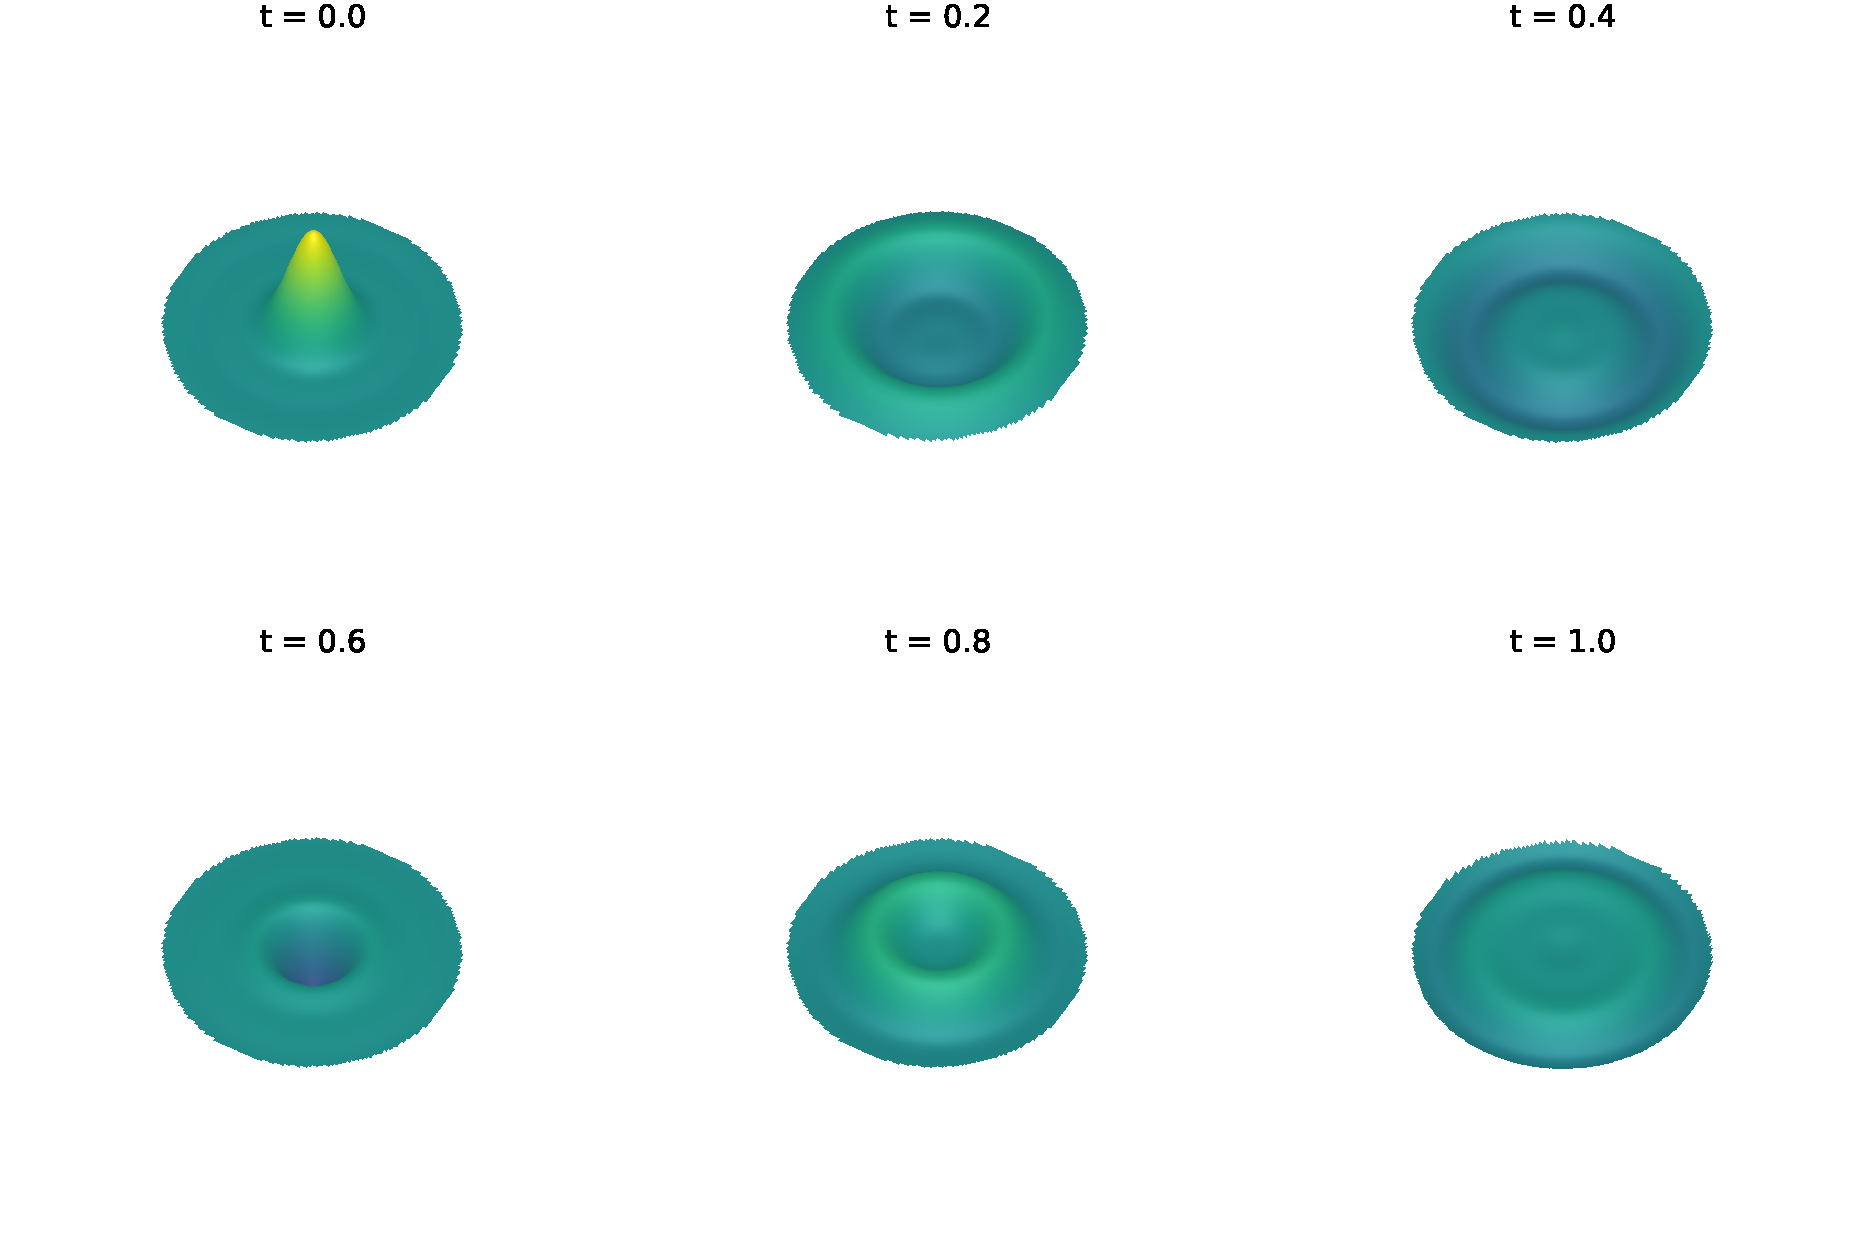
\includegraphics[width=1.0\textwidth]{src/gaussian_timestrip.pdf}
    \caption{Time evolution of a symmetric Gaussian pulse.}
    \label{fig:gaussian}
\end{figure}

More complex behaviors arise from asymmetric initial conditions, such as an off-center impact
\begin{equation}
\begin{aligned}
f_{\text{init}}(r, \theta) &= \exp(-20(r^2 + 0.5^2 - r\cos(\theta))) \\
g_\text{init}(r, \theta) &= 0.0
\end{aligned}
\end{equation}
which evolves as seen in Figure \ref{fig:offcenter}:
\begin{figure}[H]
    \centering
    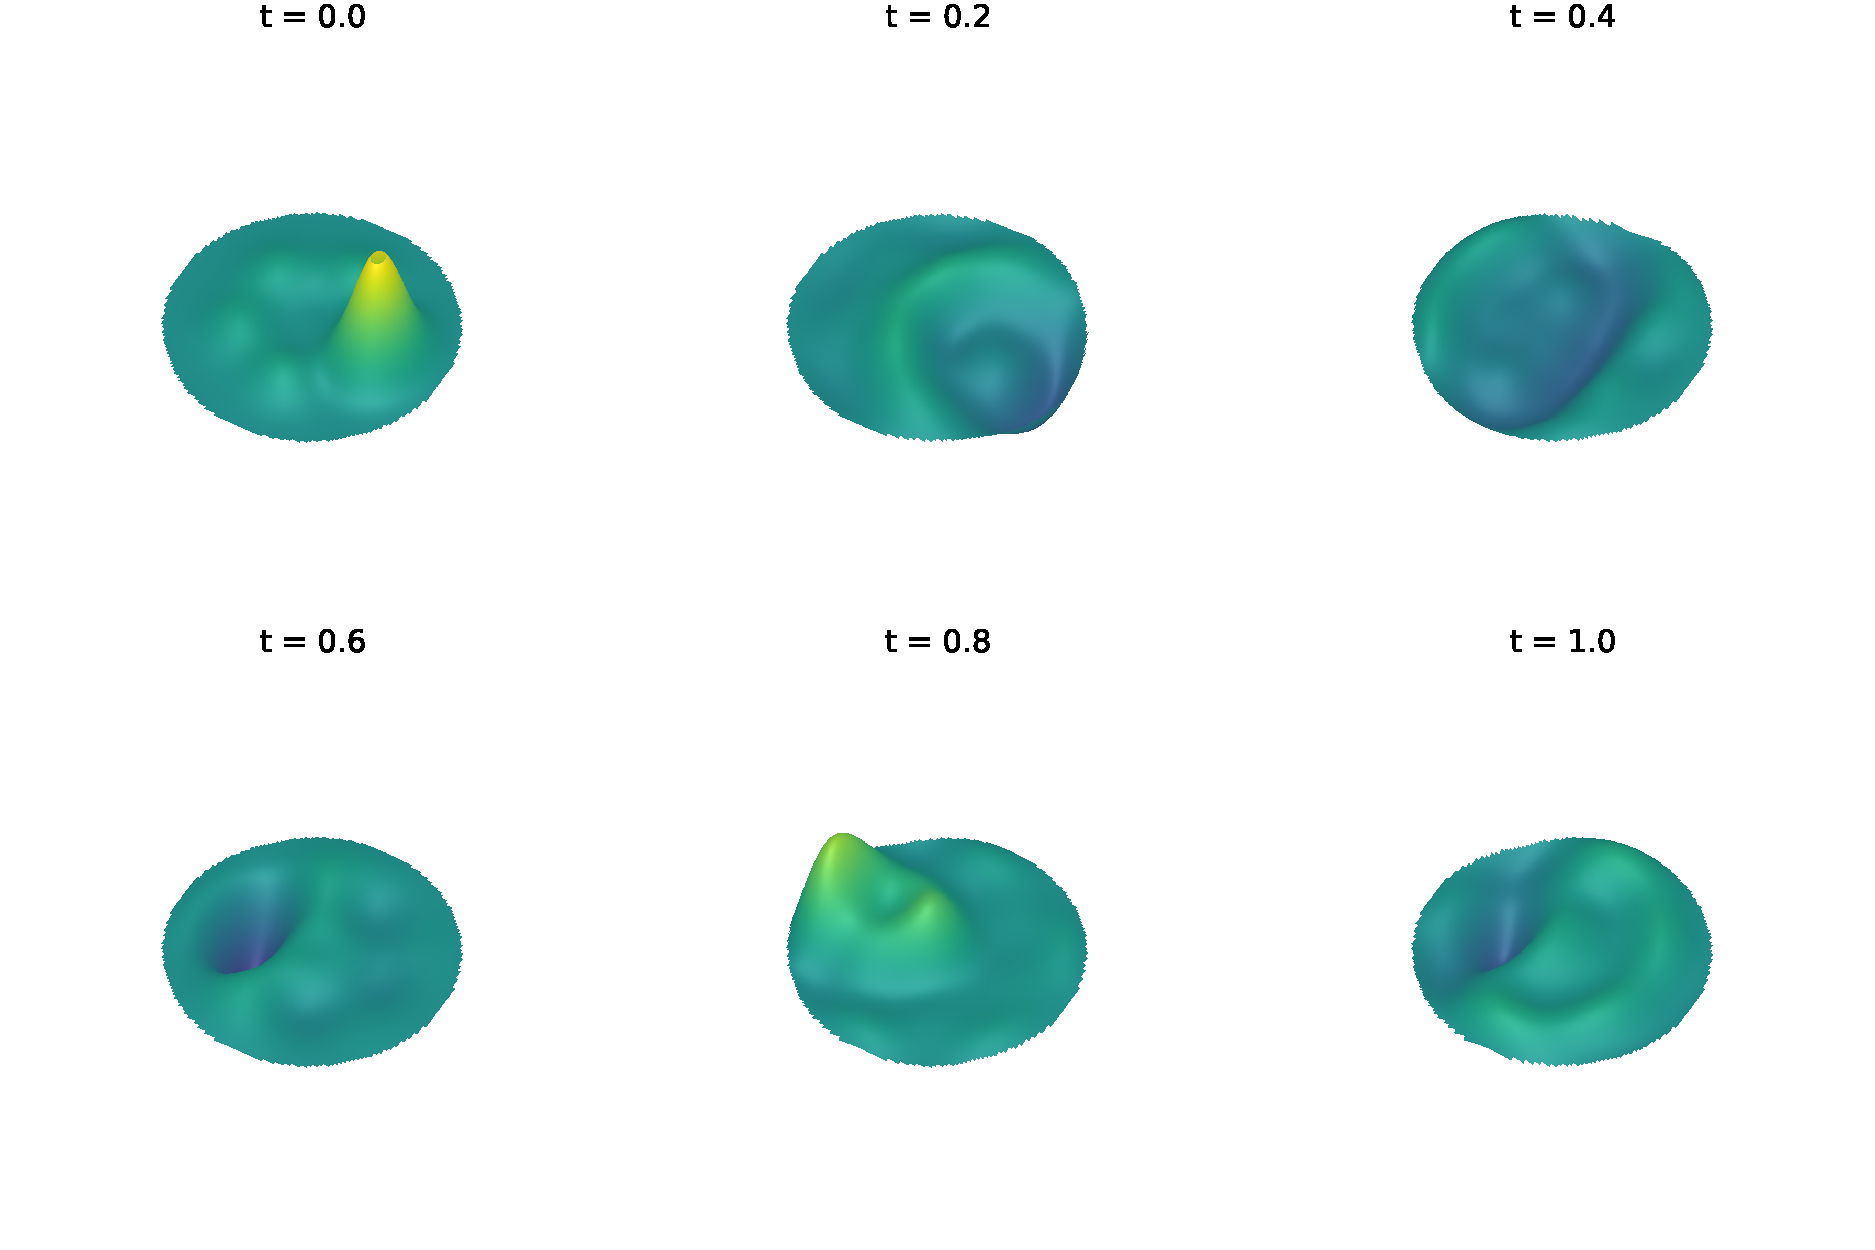
\includegraphics[width=1.0\textwidth]{src/offcenter_timestrip.pdf}
    \caption{Time evolution of an off-center strike.}
    \label{fig:offcenter}
\end{figure}

The evolution continues in this dramatic fashion indefinitely. You can find an animation on the \href{https://github.com/TonehavenE/PHYS616_Final_project}{project GitHub}.

\section{Forced Oscillations}

Thus far, we have considered the drum head in isolation, vibrating solely due to initial displacements or velocities. We now extend our analysis to consider a drum driven by an external force, such as a loudspeaker placed beneath the membrane.

\subsection{The Inhomogeneous Wave Equation}

We return to Newton's Second Law on the differential patch. Previously, the only vertical forces acting on the patch were the components of the internal tension. We now introduce an external vertical force per unit area, denoted $F_{\text{ext}}(r, \theta, t)$.

The sum of forces in the $z$-direction becomes:
\begin{equation}
    \sum F_z = F_{\text{tension}} + F_{\text{external}}
\end{equation}
Substituting our previous result for tension and applying Newton's law ($ma = \sum F$):
\begin{equation}
    (\sigma \Delta x \Delta y) \pdv[2]{u}{t} = (T \Delta x \Delta y) \nabla^2 u + (F_{\text{ext}} \Delta x \Delta y)
\end{equation}
Dividing by the mass element $\sigma \Delta x \Delta y$ and rearranging terms, we arrive at the \textbf{inhomogeneous wave equation}:
\begin{equation}
    \pdv[2]{u}{t} - c^2 \nabla^2 u = \frac{F_{\text{ext}}}{\sigma}
    \label{eq:forced_wave}
\end{equation}
where $c = \sqrt{T/\sigma}$ is the wave speed.

\subsection{Eigenfunction Expansion}

We cannot use simple separation of variables for Equation \ref{eq:forced_wave} because the equation is not homogeneous. Instead, we utilize the method of \textit{eigenfunction expansion}.

We know that the spatial modes $\psi_{mn}(r, \theta) = J_m(\lambda_{mn}r)\cos(m\theta)$ (and the corresponding sine terms) form a complete orthogonal basis for functions on the disk. Therefore, the solution $u(r, \theta, t)$ --- whatever it may be --- can be written as a sum of these modes with time-dependent coefficients.

We define the spatial mode shapes as:
\begin{equation}
    \psi_{mn}(r, \theta) = J_m(\lambda_{mn} r) \cos(m\theta)
\end{equation}

We assume a solution of the form:

\begin{equation}
    u(r, \theta, t) = \sum_{m=0}^\infty \sum_{n=1}^\infty T_{mn}(t) \psi_{mn}(r, \theta)
\end{equation}

Substituting this ansatz into the LHS of Equation \ref{eq:forced_wave}, and recalling that $\nabla^2 \psi_{mn} = -\lambda_{mn}^2 \psi_{mn}$:

\begin{align}
    \pdv[2]{u}{t} - c^2 \nabla^2 u &= \sum_{m,n} \left[ \ddot{T}_{mn}(t) \psi_{mn} - c^2 T_{mn}(t) \nabla^2 \psi_{mn} \right] \\
    &= \sum_{m,n} \left[ \ddot{T}_{mn}(t) + c^2 \lambda_{mn}^2 T_{mn}(t) \right] \psi_{mn}(r, \theta)
\end{align}

We recognize $c^2 \lambda_{mn}^2$ as the square of the natural frequency $\omega_{mn}^2$. Thus, the wave equation becomes:

\begin{equation}
    \sum_{m,n} \left[ \ddot{T}_{mn}(t) + \omega_{mn}^2 T_{mn}(t) \right] \psi_{mn}(r, \theta) = \frac{F_{\text{ext}}(r, \theta, t)}{\sigma}
\end{equation}

\subsection{Isolating the Time Dependence}

To solve for the time coefficient $T_{mn}(t)$, we exploit the orthogonality of the Bessel functions. We multiply both sides by a specific mode $\psi_{pq}(r, \theta)$ and integrate over the area of the drum $\mathcal{D}$. Due to orthogonality, all terms in the sum vanish except where $(m,n) = (p,q)$.

\begin{equation}
    \left[ \ddot{T}_{mn} + \omega_{mn}^2 T_{mn} \right] \iint_{\mathcal{D}} \psi_{mn}^2 \, dA = \frac{1}{\sigma} \iint_{\mathcal{D}} F_{\text{ext}} \psi_{mn} \, dA
\end{equation}

Let $||\psi_{mn}||^2$ denote the norm of the spatial mode (which we calculated in the Coefficient Determination section). We can now write a generic Ordinary Differential Equation (ODE) for the time evolution of each mode:

\begin{equation}
    \ddot{T}_{mn}(t) + \omega_{mn}^2 T_{mn}(t) = \frac{1}{\sigma ||\psi_{mn}||^2} \iint_{\mathcal{D}} F_{\text{ext}}(r, \theta, t) \psi_{mn}(r, \theta) \, dA
\end{equation}

This equation describes a \textbf{driven harmonic oscillator}, just as we covered in PHYS 616.

\subsection{Harmonic Forcing}

Let us consider the specific case of a speaker playing a pure tone of frequency $\Omega$. We assume the force is separable:
\begin{equation}
    F_{\text{ext}}(r, \theta, t) = P(r, \theta) \cos(\Omega t)
\end{equation}

where $P(r, \theta)$ is the spatial pressure profile of the speaker (e.g., a Gaussian concentrated at the center). The projection of the force onto the mode is:

\begin{equation}
    f_{mn} = \frac{1}{\sigma ||\psi_{mn}||^2} \iint_{\mathcal{D}} P(r, \theta) \psi_{mn}(r, \theta) \, dA
\end{equation}

Our ODE simplifies to:

\begin{equation}
    \ddot{T}_{mn}(t) + \omega_{mn}^2 T_{mn}(t) = f_{mn} \cos(\Omega t)
\end{equation}

\subsection{Solution of the Driven Oscillator}

The general solution to this ODE consists of a homogeneous part (the natural ringing of the drum) and a particular part (the response to the speaker).

\begin{equation}
    T_{mn}(t) = \underbrace{A \cos(\omega_{mn} t) + B \sin(\omega_{mn} t)}_{\text{Transient / Free}} + \underbrace{C \cos(\Omega t)}_{\text{Steady State}}
\end{equation}

Substituting $C \cos(\Omega t)$ into the ODE to find the constant $C$:

\begin{align}
    -C\Omega^2 \cos(\Omega t) + C\omega_{mn}^2 \cos(\Omega t) &= f_{mn} \cos(\Omega t) \\
    C(\omega_{mn}^2 - \Omega^2) &= f_{mn} \\
    C &= \frac{f_{mn}}{\omega_{mn}^2 - \Omega^2}
\end{align}

What this means physically is that each mode (visualized in \ref{fig:modes}) will have a different response to the driving frequency.
We can visualize how the different modes respond by plotting the amplitude of $C_{mn}$ as a function of $\Omega$:

\begin{figure}[H]
    \centering
    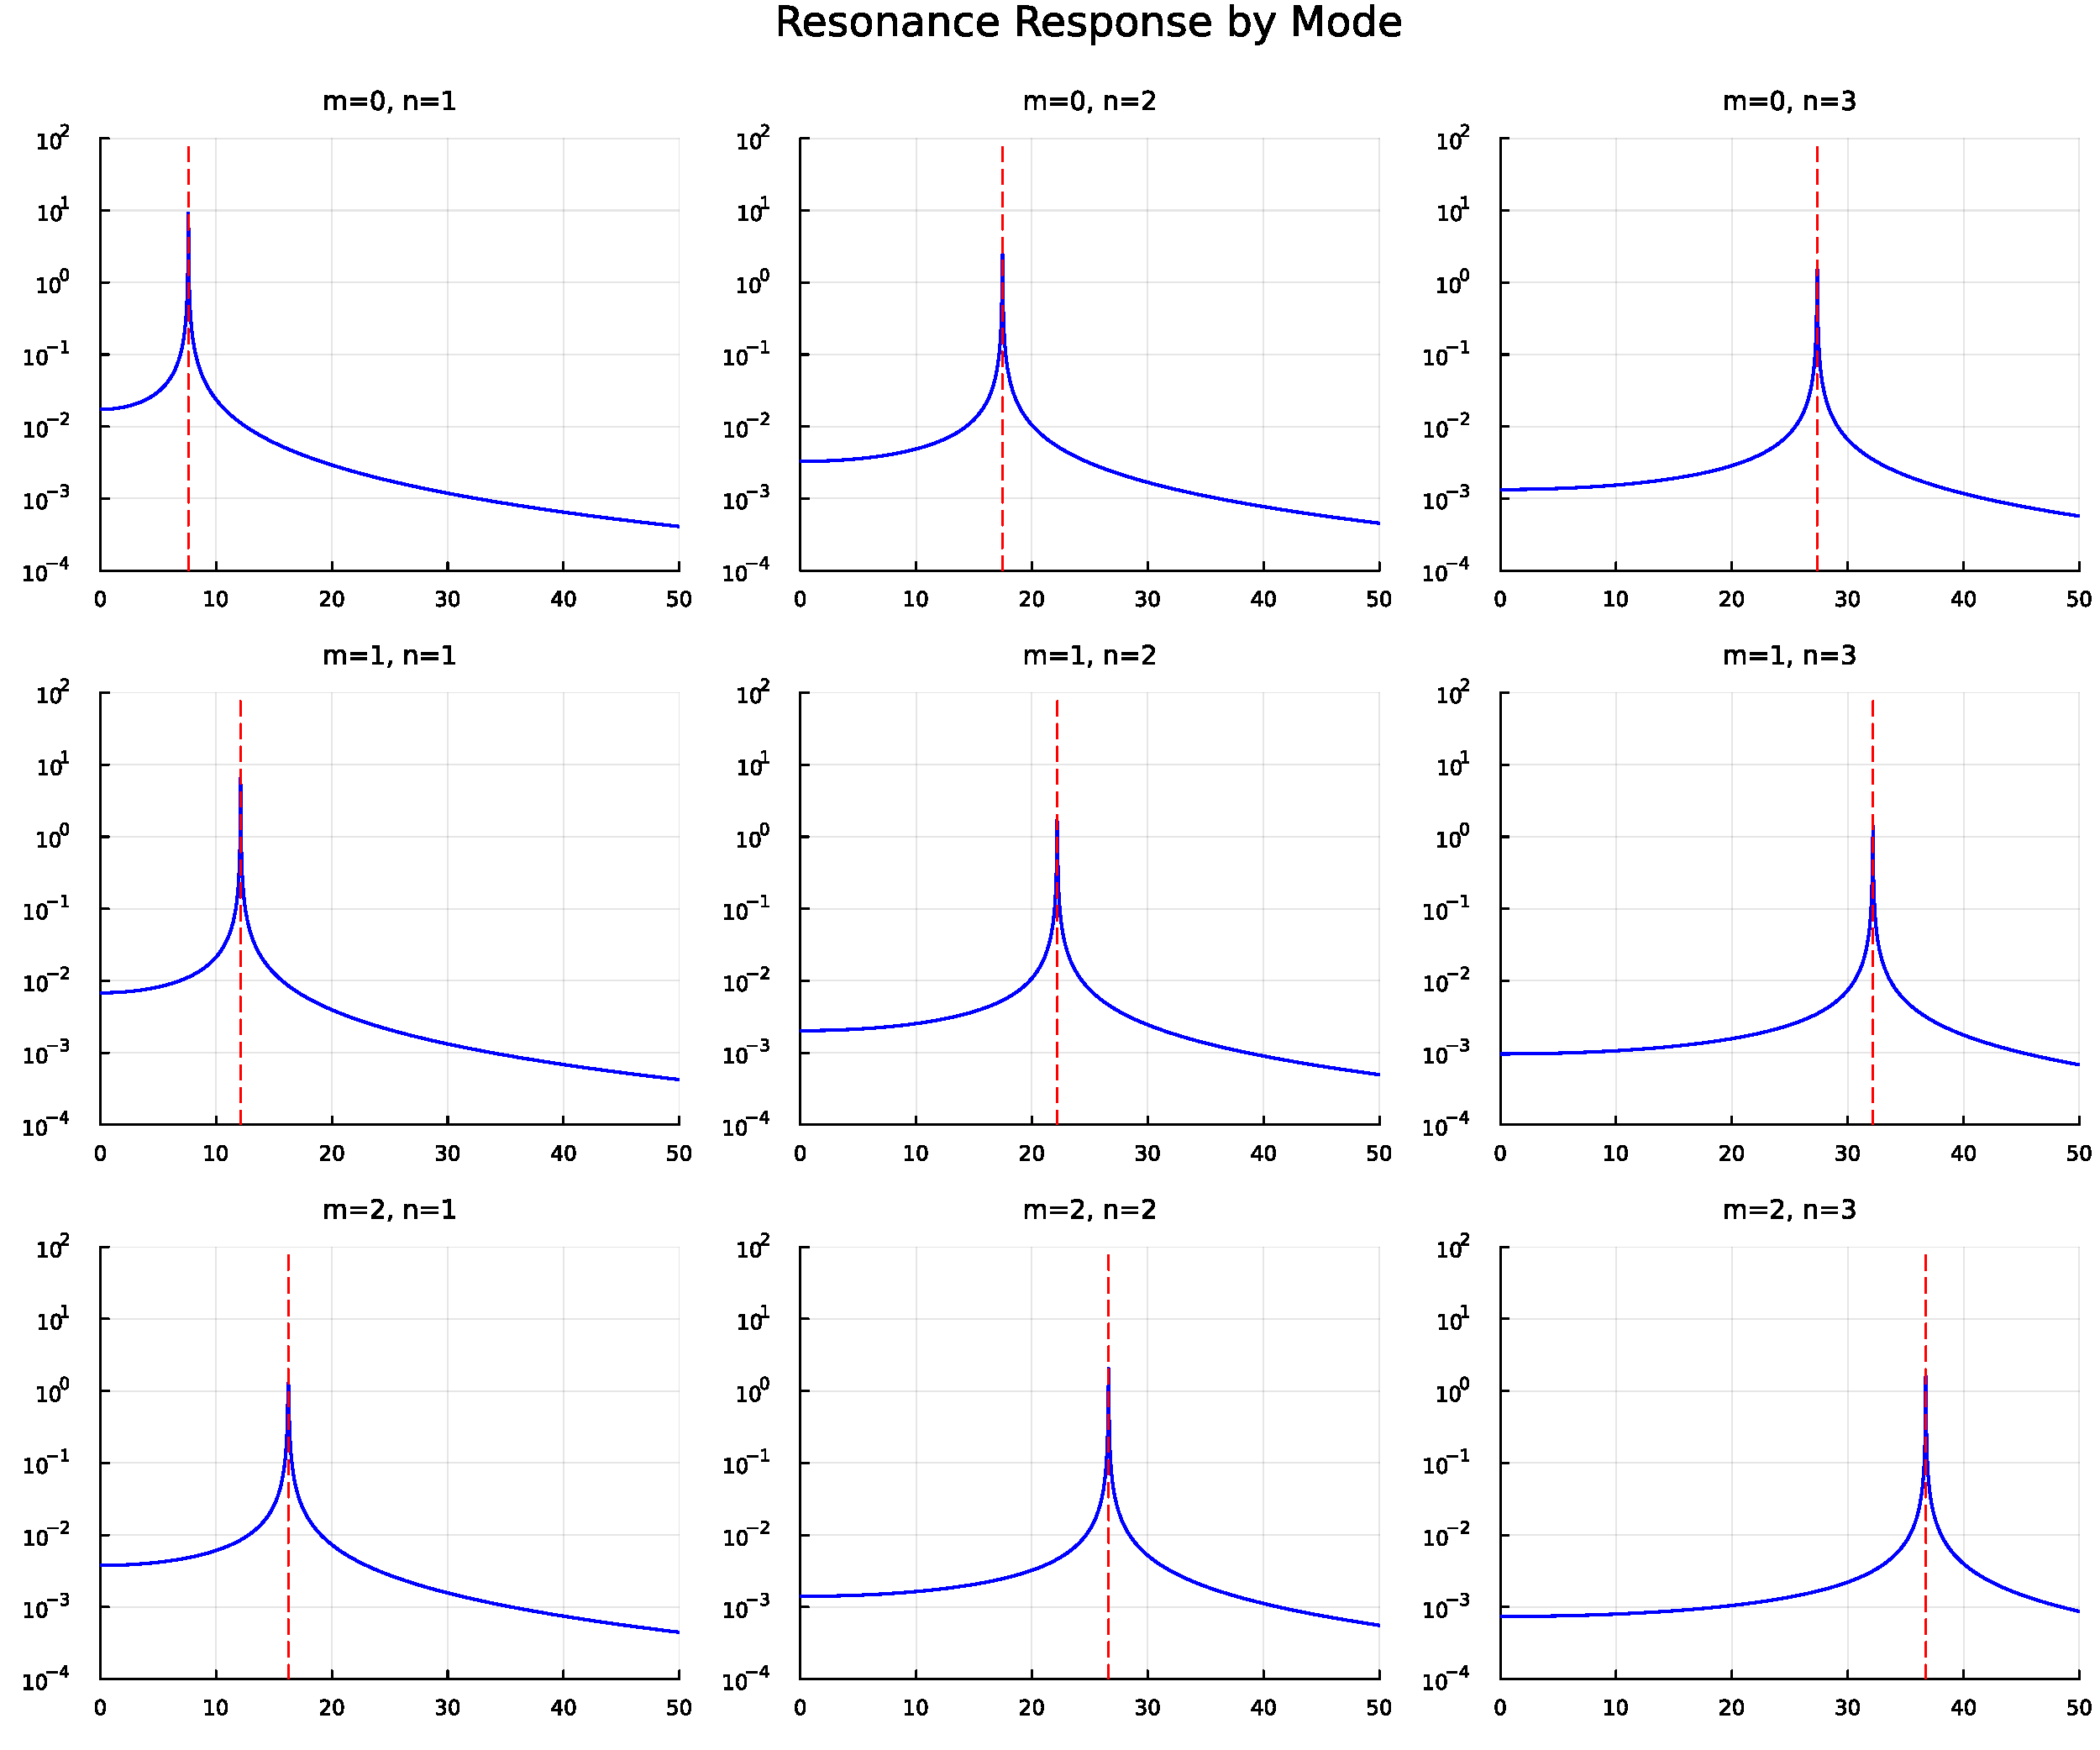
\includegraphics[width=1.0\textwidth]{src/resonances.pdf}
    \caption{Resonances for different normal modes.}
    \label{fig:resonances}
\end{figure}

If we assume the drum starts from rest ($u=0$ and $\dot{u}=0$ at $t=0$), we can solve for $A$ and $B$.
\begin{align}
    T_{mn}(0) &= A + C = 0 \implies A = -C \\
    \dot{T}_{mn}(0) &= B\omega_{mn} = 0 \implies B = 0
\end{align}

Thus, the time evolution of a specific mode under harmonic forcing is:

\begin{equation}
    \boxed{T_{mn}(t) = \frac{f_{mn}}{\omega_{mn}^2 - \Omega^2} \left[ \cos(\Omega t) - \cos(\omega_{mn} t) \right]}
\end{equation}

This result reveals the phenomenon of \textbf{resonance}. As the driving frequency $\Omega$ approaches the natural frequency of a mode $\omega_{mn}$, the denominator approaches zero, and the amplitude of that mode grows theoretically infinite (or, in reality, until damping or non-linearities dominate).

\subsection{Visualizing Driven Drums}

As with the undriven drum, we can visualize timeseries evolution of the drum. Consider a forcing function $F(r, \theta, t) \propto e^{-r^2} \cos(\Omega t)$.
If we set $\Omega$ to a resonant frequency, we see the corresponding mode become dominant. The time evolution from a drum initially at rest with a resonant frequency is shown in Figure \ref{fig:resonant_drum}.

\begin{figure}[H]
    \centering
    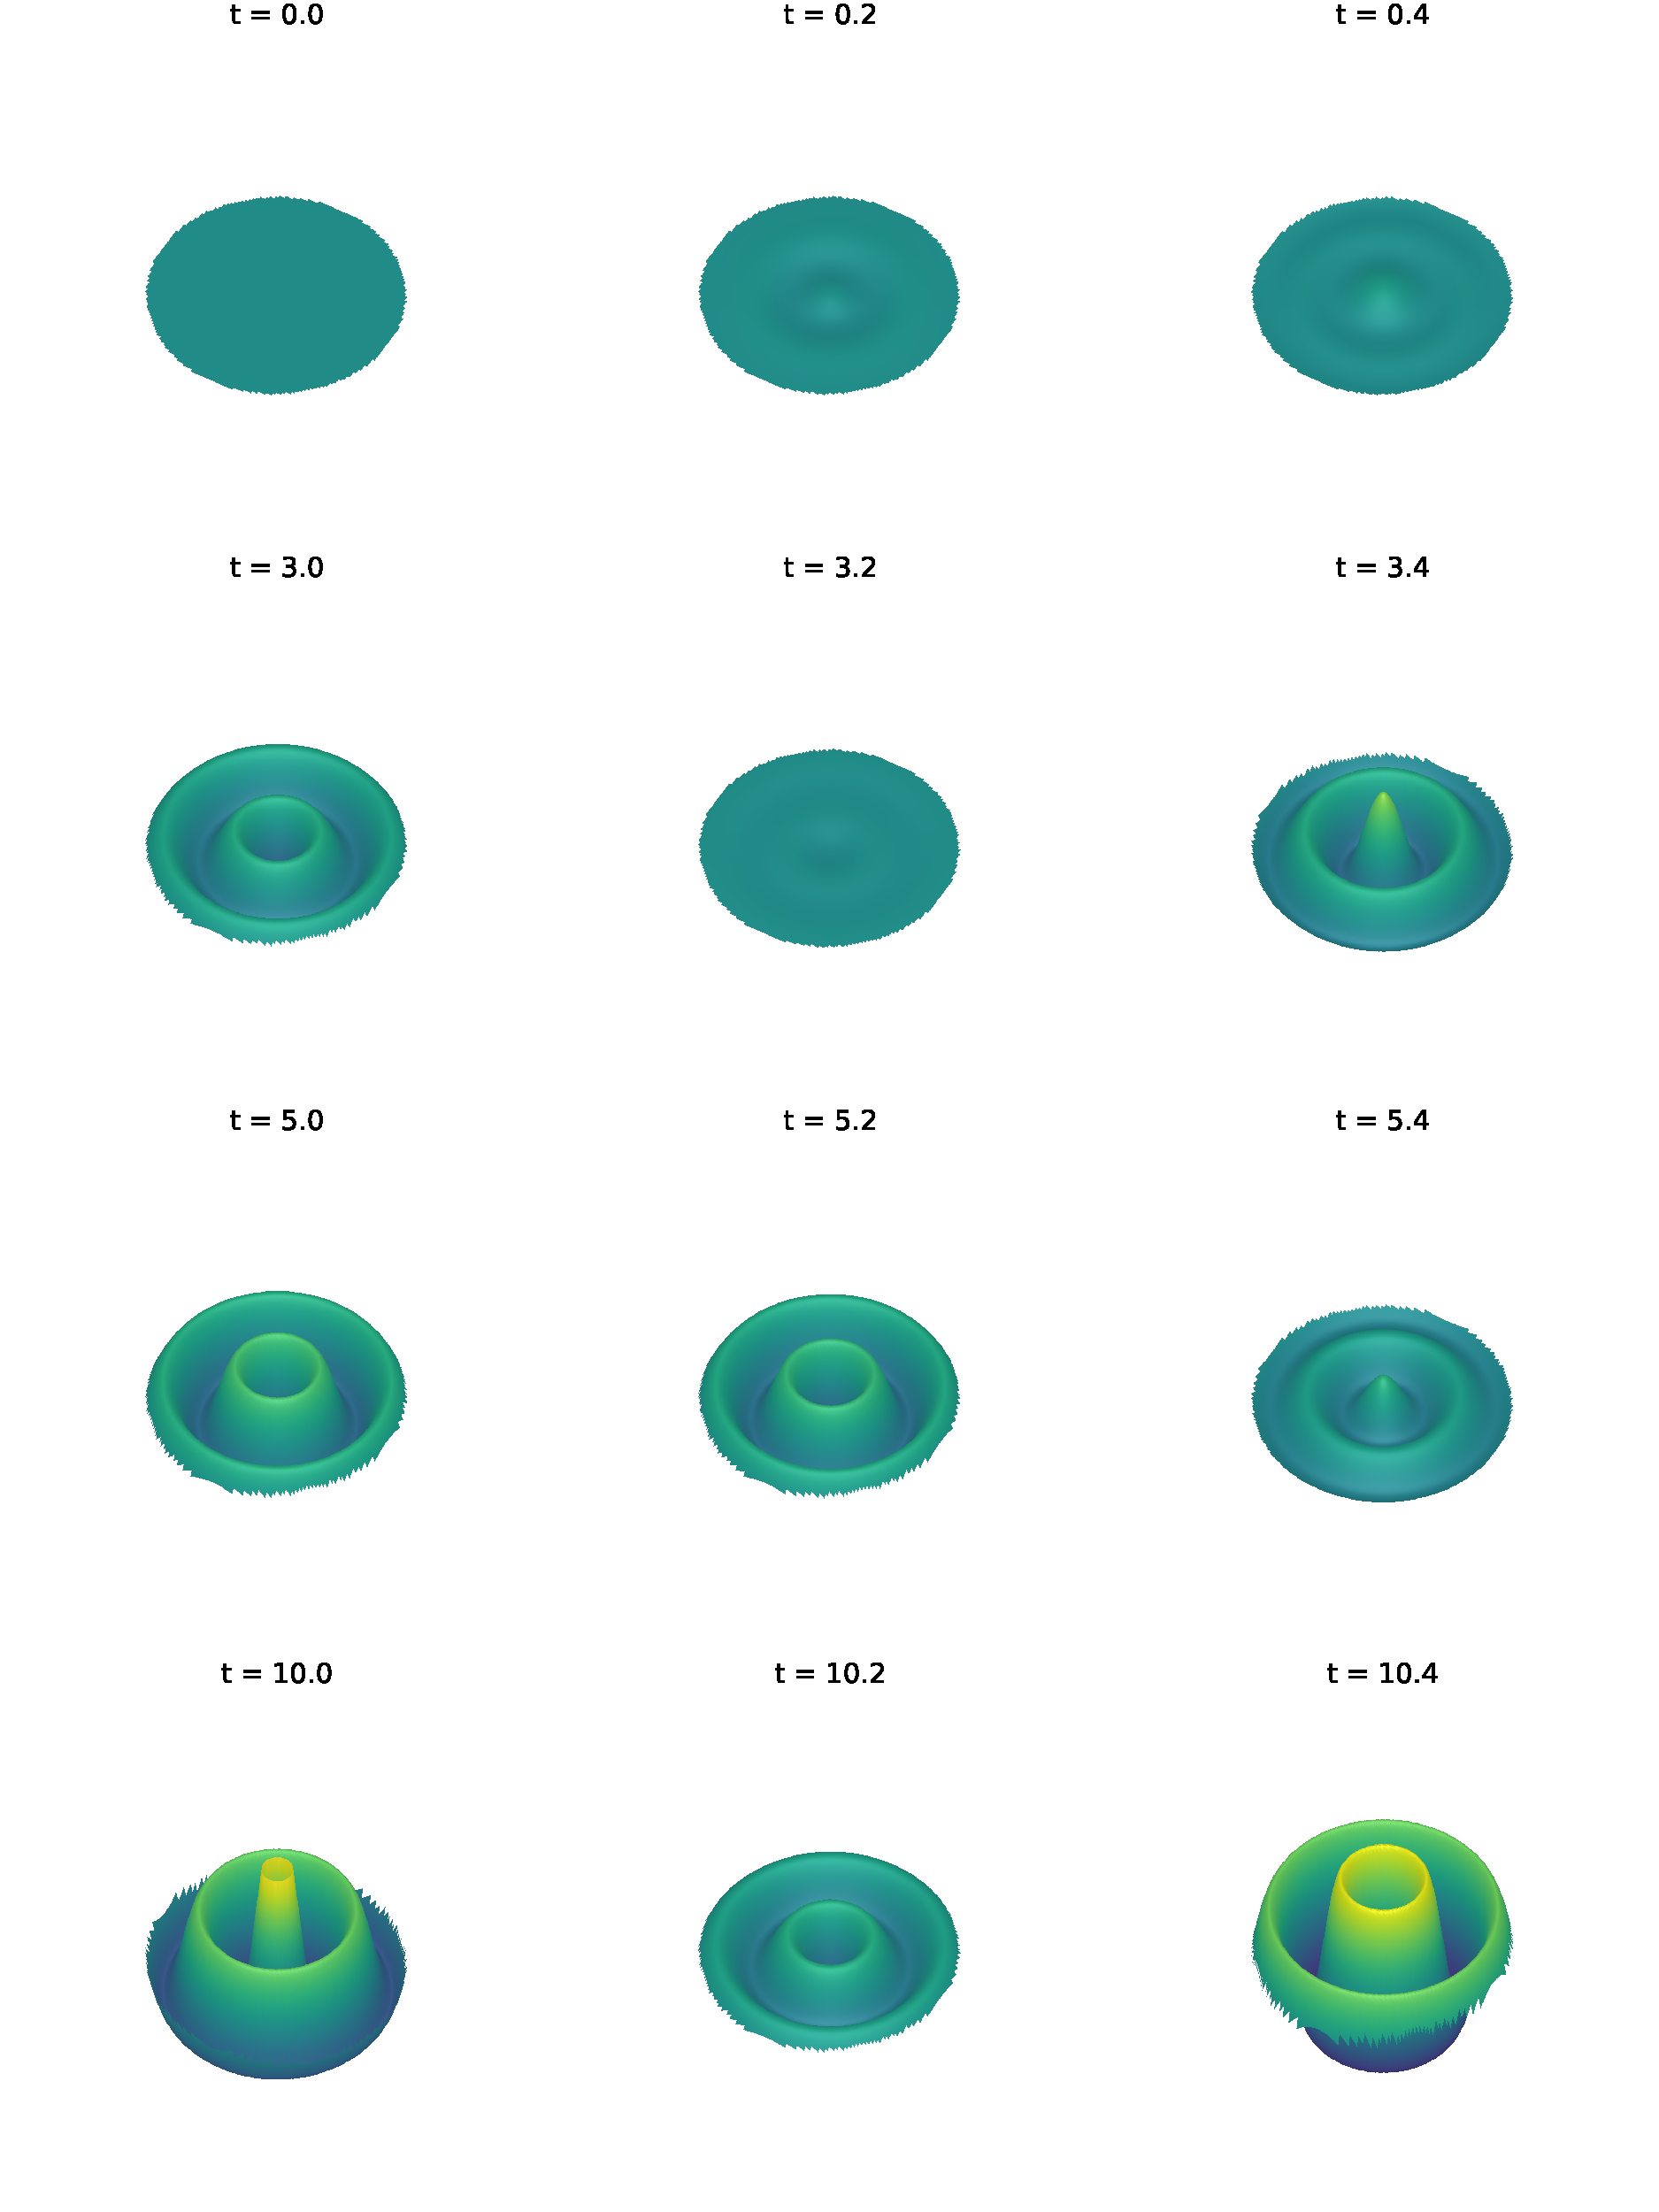
\includegraphics[max size={\textwidth}{0.7 \textheight}]{src/resonant_drum_timestrip.pdf}
	\caption{The time evolution of a drum initially at rest forced with a resonant $\Omega = 37.288 \text{Hz}$.}
    \label{fig:resonant_drum}
\end{figure}

We see the dominant mode's amplitude grow with time.
This is better visualized as an animation, which can be found in the \href{https://github.com/TonehavenE/PHYS616_Final_project}{project GitHub}.

\section{Further Studies}

There are many directions this project could be extended. 

\begin{itemize}
    \item \textbf{Non-uniform Tension:} Simulating a drum where tension varies along the boundary (common in tuning lugs).
    \item \textbf{Polygonal Geometries:} Analyzing eigenmodes of triangular or hexagonal membranes.
	\item{\textbf{Physical Experiment}: Setting up a membrane with a speaker beneath it and test how different frequencies cause responses.}
\end{itemize}

\subsection{Reflections}

It was a pleasure to work out some continuum mechanics and prove to myself where the Wave Equation comes from and why it is suitable for this problem.
It was good to exercise my skills with animations and visualization in the full code. I hope you can forgive the length of this document. 

\newpage

\appendix
\section{Derivation of the Laplacian in Polar Coordinates}

To derive the Laplacian in polar coordinates, we define $x = r \cos(\theta)$ and $y = r \sin(\theta)$. By the multivariable chain rule, the differential operators transform as:

\begin{equation}
\pdv{x} = \pdv{r}{x} \pdv{r} + \pdv{\theta}{x} \pdv{\theta}, \quad\quad \pdv{y} = \pdv{r}{y} \pdv{r} + \pdv{\theta}{y} \pdv{\theta}
\end{equation}

Computing the partials of the coordinates, we obtain:
\begin{align}
\pdv{x} &= \cos(\theta) \pdv{r} - \frac{\sin(\theta)}{r} \pdv{\theta} \\
\pdv{y} &= \sin(\theta) \pdv{r} + \frac{\cos(\theta)}{r}\pdv{\theta}
\end{align}

It is convenient to introduce the shorthand notation $\partial_{r} = \pdv{r}$ and $\partial_\theta = \pdv{\theta}$. For smooth coefficient functions $p,q$ and commuting partials $\partial_r,\partial_\theta$, we utilize the operator product rule identity:
\begin{equation}
(p\partial_i)(q\partial_j) = p q\,\partial_i\partial_j + p(\partial_i q)\,\partial_j, \qquad i,j\in\{r,\theta\}
\end{equation}

We define the coefficients for the linear operators as:
\begin{equation}
A=\cos\theta,\quad B=-\dfrac{\sin\theta}{r},\quad C=\sin\theta,\quad D=\dfrac{\cos\theta}{r}
\end{equation}

We now expand the second derivative with respect to $x$:
\begin{align*}
\partial_x^2 &= (A\partial_r + B\partial_\theta)^2 \\[4pt]
&= (A\partial_r)(A\partial_r) + (A\partial_r)(B\partial_\theta) + (B\partial_\theta)(A\partial_r) + (B\partial_\theta)(B\partial_\theta)\\[6pt]
&= A^2\partial_r^2 \;+\; A(\partial_r A)\,\partial_r \;+\; AB\,\partial_r\partial_\theta \;+\; A(\partial_r B)\,\partial_\theta \\[4pt]
&\quad +\; BA\,\partial_\theta\partial_r \;+\; B(\partial_\theta A)\,\partial_r \;+\; B^2\partial_\theta^2 \;+\; B(\partial_\theta B)\,\partial_\theta
\end{align*}

Similarly, for the second derivative with respect to $y$:
\begin{align*}
\partial_y^2 &= (C\partial_r + D\partial_\theta)^2 \\[4pt]
&= C^2\partial_r^2 \;+\; C(\partial_r C)\,\partial_r \;+\; CD\,\partial_r\partial_\theta \;+\; C(\partial_r D)\,\partial_\theta \\[4pt]
&\quad +\; DC\,\partial_\theta\partial_r \;+\; D(\partial_\theta C)\,\partial_r \;+\; D^2\partial_\theta^2 \;+\; D(\partial_\theta D)\,\partial_\theta
\end{align*}

Next, we evaluate the derivatives of the coefficients:
\begin{align*}
\partial_r A &= 0, & \partial_\theta A &= -\sin\theta, \\
\partial_r B &= \frac{\sin\theta}{r^2}, & \partial_\theta B &= -\frac{\cos\theta}{r}, \\
\partial_r C &= 0, & \partial_\theta C &= \cos\theta, \\
\partial_r D &= -\frac{\cos\theta}{r^2}, & \partial_\theta D &= -\frac{\sin\theta}{r}.
\end{align*}

Summing the two second derivatives $\nabla^2 = \partial_x^2 + \partial_y^2$ and collecting terms by operator:
\begin{align*}
\nabla^2 &= (A^2+C^2)\partial_r^2 + (B^2+D^2)\partial_\theta^2 + 2(AB+CD)\partial_r\partial_\theta \\[4pt]
&\quad +\big[A(\partial_r A)+B(\partial_\theta A)+C(\partial_r C)+D(\partial_\theta C)\big]\partial_r \\[4pt]
&\quad +\big[A(\partial_r B)+B(\partial_\theta B)+C(\partial_r D)+D(\partial_\theta D)\big]\partial_\theta
\end{align*}

We evaluate the bracketed coefficients term by term:
\begin{align*}
\textbf{1. } & A^2+C^2 = \cos^2\theta+\sin^2\theta = 1 \\[6pt]
\textbf{2. } & B^2+D^2 = \frac{\sin^2\theta}{r^2}+\frac{\cos^2\theta}{r^2} = \frac{1}{r^2} \\[6pt]
\textbf{3. } & AB+CD = \cos\theta\left(-\frac{\sin\theta}{r}\right)+\sin\theta\left(\frac{\cos\theta}{r}\right) = 0 \\[6pt]
\textbf{4. } & [\dots]\partial_r = 0 + \left(-\frac{\sin\theta}{r}\right)(-\sin\theta) + 0 + \left(\frac{\cos\theta}{r}\right)\cos\theta = \frac{\sin^2\theta + \cos^2\theta}{r} = \frac{1}{r} \\[6pt]
\textbf{5. } & [\dots]\partial_\theta = \frac{\sin\theta\cos\theta}{r^2} + \frac{\sin\theta\cos\theta}{r^2} - \frac{\sin\theta\cos\theta}{r^2} - \frac{\sin\theta\cos\theta}{r^2} = 0
\end{align*}

Substituting these values back into the summation, we arrive at:
\begin{equation}
\nabla^2 = \partial_r^2 + \frac{1}{r}\partial_r + \frac{1}{r^2}\partial_\theta^2
\end{equation}

Returning to standard partial derivative notation and writing the radial terms as a product rule, the Laplacian is:
\begin{equation}
\boxed{\nabla^2 = \frac{1}{r} \pdv{r} \left( r \pdv{r} \right) + \frac{1}{r^2} \pdv[2]{\theta}}
\end{equation}

\section{Properties of Bessel Functions}

In the derivation of the radial solution for the circular membrane, we encountered Bessel's Differential Equation:
\begin{equation}
    x^2 \frac{d^2 y}{dx^2} + x \frac{dy}{dx} + (x^2 - n^2)y = 0
\end{equation}
where $n$ is a non-negative integer (in our physical case, the angular mode number). The general solution to this equation is a linear combination of Bessel functions of the first kind, $J_n(x)$, and the second kind, $Y_n(x)$:
\begin{equation}
    y(x) = c_1 J_n(x) + c_2 Y_n(x)
\end{equation}

\subsection{Bessel Functions of the First Kind ($J_n$)}
Bessel functions of the first kind are finite at the origin $x=0$. They are often defined via the series expansion:
\begin{equation}
    J_n(x) = \sum_{k=0}^{\infty} \frac{(-1)^k}{k! \, \Gamma(k+n+1)} \left(\frac{x}{2}\right)^{2k+n}
\end{equation}
where $\Gamma(z)$ is the Gamma function (for integer $n$, $\Gamma(n+1) = n!$).



Alternatively, $J_n(x)$ can be defined via the \textbf{generating function}, a technique useful for deriving recurrence relations:
\begin{equation}
    e^{\frac{x}{2}(t - 1/t)} = \sum_{n=-\infty}^{\infty} J_n(x) t^n
\end{equation}
Physically, $J_n(x)$ represents a decaying standing wave in the radial direction.

\subsection{Bessel Functions of the Second Kind ($Y_n$)}
The Bessel function of the second kind (also known as the Weber or Neumann function) is defined as:
\begin{equation}
    Y_n(x) = \lim_{\nu \to n} \frac{J_\nu(x) \cos(\nu \pi) - J_{-\nu}(x)}{\sin(\nu \pi)}
\end{equation}
A crucial property for physical applications is the behavior near the origin. As $x \to 0$:
\begin{equation}
    Y_n(x) \sim \begin{cases} 
    \frac{2}{\pi} \ln(x/2) & n=0 \\ 
    -\frac{(n-1)!}{\pi} \left(\frac{2}{x}\right)^n & n > 0 
    \end{cases}
\end{equation}


Because $Y_n(x) \to -\infty$ as $x \to 0$, it represents a solution with infinite displacement at the center of the drum. This is physically impossible for a continuous membrane, compelling us to set the coefficient $c_2 = 0$.

\subsection{Orthogonality}
The Fourier-Bessel series expansion relies on the orthogonality of Bessel functions. For a fixed order $n$, the set of functions $\{J_n(\lambda_{nk} r)\}$ forms an orthogonal basis on the interval $[0, a]$ with respect to the weight function $w(r) = r$.

Let $\alpha_{nk}$ and $\alpha_{nm}$ be two distinct roots of $J_n(x) = 0$. Then:
\begin{equation}
    \int_0^a J_n\left(\frac{\alpha_{nk}}{a} r\right) J_n\left(\frac{\alpha_{nm}}{a} r\right) r \, dr = 0 \quad \text{if } k \neq m
\end{equation}

If $k = m$, we obtain the normalization constant:
\begin{equation}
    \int_0^a \left[ J_n\left(\frac{\alpha_{nk}}{a} r\right) \right]^2 r \, dr = \frac{a^2}{2} [J_{n+1}(\alpha_{nk})]^2
\end{equation}
This identity allows us to isolate the coefficients $A_{mn}$ and $B_{mn}$ in the general solution.

\subsection{Roots and Zeros}
The boundary condition $u(a, \theta, t) = 0$ requires that $J_n(\lambda a) = 0$. The function $J_n(x)$ has an infinite number of real, positive roots. We denote $\alpha_{nk}$ as the $k$-th zero of $J_n(x)$.
\begin{itemize}
    \item For $n=0$: Roots correspond to symmetric modes (breathing modes).
    \item For $n>0$: Roots correspond to modes with diametric nodes.
\end{itemize}
For large $k$, the roots are approximately evenly spaced by $\pi$:
\begin{equation}
    \alpha_{nk} \approx \left(n + \frac{1}{2} + 2k\right)\frac{\pi}{2}
\end{equation}

\newpage

\begin{thebibliography}{9}

\bibitem{errede}
Errede, S. (2017). \textit{Acoustical Physics of Music: Vibrations of Ideal Circular Membranes}. UIUC Physics 406.

\bibitem{russell}
Russell, D. (2018). \textit{Mode Shapes of a Circular Membrane}. Pennsylvania State University.

\bibitem{wolfram}
Weisstein, E. W. \textit{Bessel Function of the First Kind}. MathWorld--A Wolfram Web Resource.

\end{thebibliography}

\end{document}
